\documentclass[a4paper]{article}

\usepackage[pages=all, color=black, position={current page.south}, placement=bottom, scale=1, opacity=1, vshift=5mm]{background}
\SetBgContents{
	\tt Adam Zawieruhca
}      

\usepackage[margin=1in]{geometry} % full-width

% AMS Packages
\usepackage{amsmath}
\usepackage{amsthm}
\usepackage{amssymb}

% Unicode s
\usepackage[utf8]{inputenc}
\usepackage{hyperref}
\hypersetup{
	unicode,
%	colorlinks,
%	breaklinks,
%	urlcolor=cyan, 
%	linkcolor=blue, 
	pdfauthor={Author One, Author Two, Author Three},
	pdftitle={A simple article template},
	pdfsubject={A simple article template},
	pdfkeywords={article, template, simple},
	pdfproducer={LaTeX},
	pdfcreator={pdflatex}
}

% Vietnamese
%\usepackage{vntex}

% Natbib
\usepackage[sort&compress,numbers,square]{natbib}
\bibliographystyle{mplainnat}

% Theorem, Lemma, etc
\theoremstyle{plain}
\newtheorem{theorem}{Theorem}
\newtheorem{corollary}[theorem]{Corollary}
\newtheorem{lemma}[theorem]{Lemma}
\newtheorem{claim}{Claim}[theorem]
\newtheorem{axiom}[theorem]{Axiom}
\newtheorem{conjecture}[theorem]{Conjecture}
\newtheorem{fact}[theorem]{Fact}
\newtheorem{hypothesis}[theorem]{Hypothesis}
\newtheorem{assumption}[theorem]{Assumption}
\newtheorem{proposition}[theorem]{Proposition}
\newtheorem{criterion}[theorem]{Criterion}
\theoremstyle{definition}
\newtheorem{definition}[theorem]{Definition}
\newtheorem{example}[theorem]{Example}
\newtheorem{remark}[theorem]{Remark}
\newtheorem{problem}[theorem]{Problem}
\newtheorem{principle}[theorem]{Principle}

\usepackage{graphicx, color}
\graphicspath{{fig}}

%\usepackage[linesnumbered,ruled,vlined,commentsnumbered]{algorithm2e} % use algorithm2e for typesetting algorithms
\usepackage{algorithm, algpseudocode} % use algorithm and algorithmicx for typesetting algorithms
\usepackage{mathrsfs} % for \mathscr command

\usepackage{lipsum}

% Author info
\title{Minimizing Page Faults on Bloom Filters
\author{Adam Zawierucha (adz2)}

\date{
	Rice University \\ zawie@rice.edu}%
%	\today
}


\begin{document}
	\maketitle
	
	\begin{abstract}
		Bloom filters \cite{Bloom} are used ubiquitously due to their speed and memory efficiency in theory and in practice.
However, the standard implementation of sufficiently large bloom filters suffers from page faults.
In this paper we propose a bloom filter implementation that guarantees one page access per operation. 
This minimizes page faults, thereby drasticaly improving efficiency.
We will show theoretically and empirically that our hierarchical implementation is expected to be faster than the standard implementation without alterating the false positive rate.

\noindent\textbf{Keywords:} probabilistic data structures, bloom filters, memory hierarchy, implementation, page fault analysis
	\end{abstract}
	

	\section{Introduction}
	 

	\section{Implementations}
	\newcommand{\sep}{\hspace*{0.15in}}
\newcommand\cell{%%
    \fbox{\rule{0.15in}{0pt}\rule[-0.5ex]{0pt}{0.15in}}}

\subsection{Standard Implementation}
Before we discuss the proposed solution, let us highlight the weakness of the standard implementation.
The standard implementation allocates a bit vector of size $m$ bits. Typically, this is set to be $\times 10$ the expected number of elements it will hold.
The figure below represents the bit vector of length $m$.

\begin{center}
    \textit{Standard Bloom Filter}
    \vspace{10pt}\\
    $\text{Bit Vector: } \cell\cell\cell\cell\cell\cell\cell\cell\cell\cell\cell\cell \ldots$
    \vspace{10pt}\\
    \textbf{Figure 1}
\end{center}

Per the standard implementation, to insert an element we hash the element $k$ times and set the corresponding bit in the vector.
To query, we simply read instead of set the bit.
Notice, that if $m$ is sufficiently large, it will span accross multiple pages of memory. 
Thus, when we read and write to the underlying bit vector, we may page fault for every bit set, slowing down our insertions or queries.

\subsection{Proposed Hierarchical Implementation}
Our proposal is to allocate $w$ bit vectors of size $P$ bits, where $P$ is computer system's page size in bits and $w$ is an integer such that $m = w P$.
Notice, our proposed implementation uses the same amount of memory, but  splits the bit vector into page size chunks.

\begin{center}
    \textit{Hierarchical Bloom Filter}
    \vspace{10pt}\\
    $\text{Bit Vector 1: }\cell\cell\cell\cell \sep \text{Bit Vector 2: }\cell\cell\cell\cell \sep \ldots \sep \text{Bit Vector $w$: }\cell\cell\cell\cell$
    \vspace{10pt}\\
\end{center}

To insert, hash the element $l$ times mod $w$ and insert the element per the standard bloom filter operations to the corresponding bit vector.
Each bit vector (bloom filter) has $k$ hash functions associated with it.
Here $l$ is a pre-determined parameter of the datastructure; we will dicuss what the optimal setting is in a following section.
To query, we simply query the corresponding bit vector instead of inserting.
In essence, our proposal to create a bloom filter of bloom filters, hence the name.

Notice, for any given insertion or query, we have to perform $l$ more hash operations than the standard implementation. 
This is not a concern if we select sufficiently cheap hash functions.
More importantly, ince each bit vector is on it's own page of memory, we expect to page fault at most $l$ times.
 Thus, if we minimize $l$ without sacrificing effectiveness, we will reduce the expected number of page faults and increase the data structures efficiency.

	\section{Theoretical Work}
	In this section we will justify why the hierarchical implementation will outperform the standard implementation in theory while preserving effectiveness.
First, we will \textbf{calculate expected number of page faults} for  each implementation.
Second, we will \textbf{find the theoeretical false positive rate}, which will guide us in our parameter selection for the implementation.

\subsection{Expected Page Faults}
Page faults occur when the operating system is forced to fetch data from a source lower in the memory hierarchy to be used by the process.
Whenever a page fault occurs, the program must be halted to resolve the page fault, which requires relatively slow I/O operations such as checking the TLB or loading the page from disk.
This leads to slower performance.

\begin{center}
    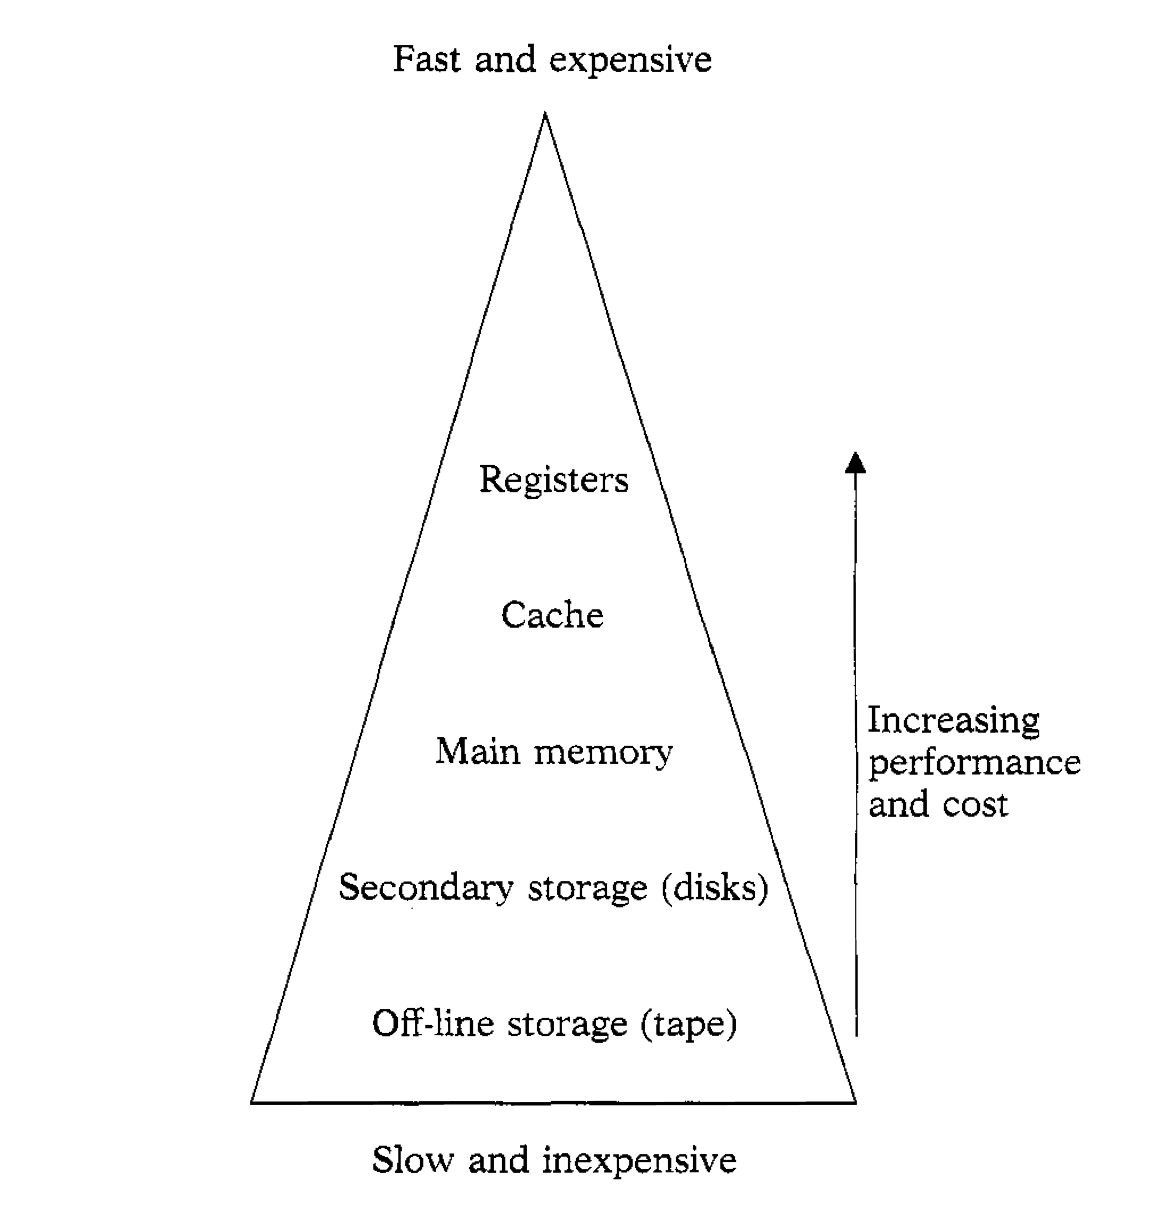
\includegraphics[width=6cm]{memHier.png}
    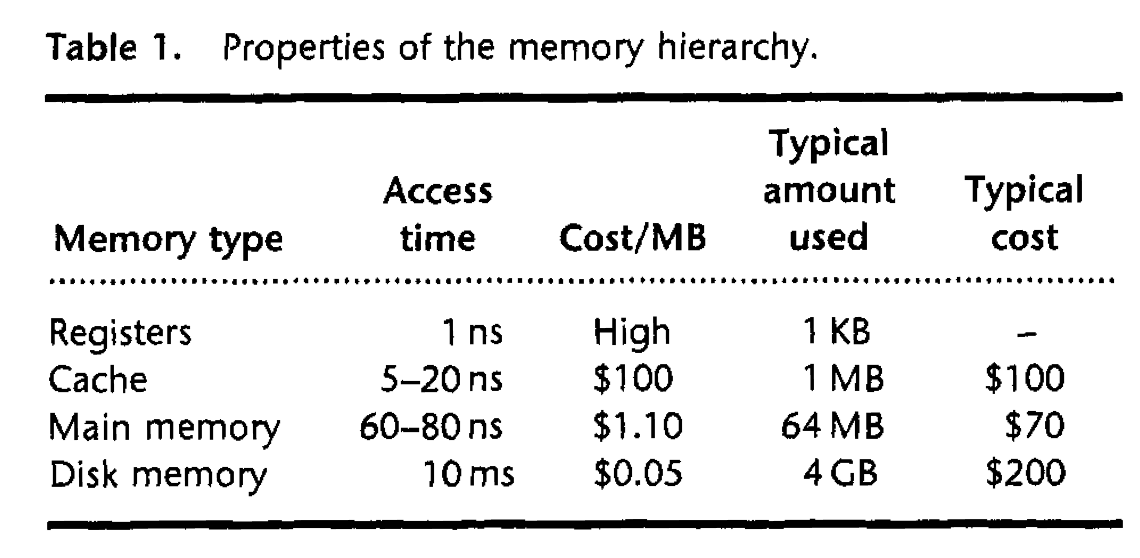
\includegraphics[width=9cm]{memTable.png}

    \cite[Murdocca et al.]{Murdocca}
\end{center}

As demonstrated in the figures above from Miles J. Murdocca et al. \cite{Murdocca}, we see that we get radically better performance the closer we access memory to the CPU.
If we design our algorithm to be more cache-efficient, then we expect massive speed-ups in practie. 

Note, when discussing page faults in this section, we will only discuss the page faults caused due to accessing the underlying bit vector of the bloom filter.
Natuarlly, page faults can occur while running the underlying code of the bloom filter, but this should be rare and would realistically cause at most one page fault.
We will now compute the expected number of page acceses for both the standard and hierarchical implementation.

The problem with doing an anaylsis on page faults is that it impossible to know when accessing a page will cause a page fault as this is dependant on the operating system and hardware.
Generally, the more memory you are using, the higher the likelyhood a page fault will occur.
In this analysis we will assume more page accesses is coorelated with a higher liklihood of page faulting.
In otherwords, we can approximate the liklihood of page page fault to the expected number of different pages that will be accessed during an operation.

First, we will discuss the standard implementation. Let $A$ be a random variable representing the number of pages accessed. 
Let $P$ be the number of bits in a page and let $m$ be the number of bits in the underlying bitvector.
Suppose there are $k$ hash functions.
We now define the indictor variable $A_i$ which is $1$ if bit $i$ is set, $0$ otherwise.
$$A = A_1 + A_2 + \ldots + A_{m/P}$$
Thus, the expected number of distinct pages accessed can be found by computing the expected value that any given page is accessed and applying linearity of expectation:
$$E(A) = \sum_{i=1}^{m/P} E(A_i) = \frac{m}{P} \cdot E(A_i) \text{ for arbitrary $i$}$$
The probability that $A_i$ is accesed at least once is the inverse of it being never accessed.
Assuming that our hash function is uniform, we expect it to pick any particular page with probability $\frac{1}{m/P} = \frac{P}{m}$.
Thus, the probablity $A_i$ is accessed at least once is:
$$E(A_i)  = 1 - (1 - \frac{P}{m})^k$$
Ergo, we have a closed form equation for the expected number of page faults for a given operation:
$$\text{Expected distinct pages accessed (Standard)} = \frac{m}{P} (1 - (1 - \frac{P}{m})^k)$$

We will use this formula to compute the expected number of page faults for two reasonable cases.
First, suppose you wanted a bloom filter to store $32,768$ elements with an underlying bit vector of size $\times 10$ that.
Note, most computer systems have a page size of $4096$ bytes, so this works out to require exactly $10$ pages of memory.
Additionally, suppose we pick the optimal bloom filter parameter and set $k=7$.
Under this scenario, we anticpate:
$$\text{Expected distinct pages accessed (Standard)} = 10(1-0.9^7) \approx 5.2$$
If we wanted to store $327,680$ elements under a similar setting, then the number of pages faults would be:
$$\text{Expected distinct pages accessed (Standard)} = 100(1-0.99^7) \approx 6.8$$

As we can see, even using a relatively small bloom filter, we anticpate almost every bit to be located in an entirely different page.
This means we can page fault multiple times during a single operation.

We will now anaylze the hierarchical implementatin. Our implementation limits bit setting and reading to a single page per insertion or query. Therefore, we access exactly one page!
$$\text{Distinct page accessed (Hierarchical)} = 1$$

Thus, our proposed hierarchical solution page faults at most one time!
Therefore, we anticpate much better performance.
\subsection{False Positive Rate}

In this section we will demonstrate that both implementations will have the same false positive rate in theory.
\subsubsection{Standard False Positive Rate}

As we have covered in class, the false positive rate of a standard bloom filter is as follows.
\begin{equation}
    (1 - (1 - \frac{1}{m})^{nk})^k \approx (1  - e)^{kn/m}
\end{equation}

Setting $k=7$ will minimize the false positive rate, as discussed in class.

\subsubsection{Hierarchical False Positive Rate}
Suppose we have a allocated $m$ bits in total chunked into bit vectors of size $P$ and that we have to inserted $n$ elements into our bloom filter.

We now want to compute the false positive rate of the hierarchical implementation.
This can be computed by supposing the bloom filter has been filled with $n$ elements and computing the probability that a querying a false key would result in a true response.

Assuming our hash function is uniform, any particular sub-bloom filter is anticpated to have $\frac{nl}{m/P} = \frac{nlP}{m} $ elements in it.
There are $m/P$ bloom filters and we choose $l$ of them to check. As before $k$ is the number of hash functions a particular bloom filter uses.
Thus, the chance any one bloom filter is set is:
$$(1-(1 - \frac{1}{P})^{lknP/m})^k$$
For our hierarchical implementation to return true, all $l$ bloom filters selected must return a positive result.
Thus, the false positive rate is:
$$((1 - \frac{1}{P})^{lknP/m})^{kl}$$
We can use a well known identity for $e^{-1}$ to approximate this false positive rate:
$$\approx (1 - e^{-lkn/m})^{lk}$$

Interestingly, this removes the dependence on the page size.
However, it is important to note that the Euler identity is $e^{-1} = \lim_{x\rightarrow\infty}(1-\frac{1}{P})^P$, so this identity fails as an approximation the smaller $P$ becomes.
Therefore, we should pick $P$ to be the largest value where we expect speed ups, which would be the size of a physical page.
More importantly, this formula becomes isomorphic to the false positive rate for the standard implementation.
If we let $k' := lk$ we see that our false positive rate for the hierarchical implementation is:
$$\approx (1 - e^{-k'/m})^{k'}$$
Therefore, as discussed for the standard implementation, the optimal selection for $k'$ is $7$.
Therefore, either $l=1$ and $k=7$ or $l=7$ and $k=1$.
Since our goal is reduce the number of pages accessed, the former is a more sensible choice.

Therefore, the best parameter selection for our hierarchical implementation would be to select $1$ bloom filter the size of a bloom filter and set $7$ bits in each one.
$$l = 1\text{ ; } k = 7$$

\subsection{Conclusion}
Our theoretical work has justified the claim that we expect this implementation to be more performant while having the same positive rate as the standard implementaiton.
Moreover, we have found the optimal parameters to use for our implementation.

	\section{Experiments}
	We will now emperically validate that the hierarchical implementation is more time efficient than the standard implementation without sacrificying accuracy.
Two experiments will be conducted.
First, we will \textbf{measure elapsed time as insertions scale} of each implementation.
We anticpate that the hierarchical implementation will take less time than the standard implementation for any sufficiently large value of insertions.
Second, we will \textbf{measure false positives as we scale bits allocated per element} of each implementation.
We anticipate that the hierarchial and standard implementation will be approximately same as the theoerical false positive rate discussed before.

For both of these sections, we pseudorandomly generate keys to both insert and query.
Discussion on exactly how these keys are generated is outlined in the appendix.

%%%%%%%%%%%%%%%%%%%%%%%%%%%%%%%%%%%%%%%%%%
%%%%%%%%%%%%%%%%%%%%%%%%%%%%%%%%%%%%%%%%%%
%%%%%%%%%%%%%%%%%%%%%%%%%%%%%%%%%%%%%%%%%%

\subsection{Comparing Time Efficiency}

For this experiment, we seek to validate that the hierarchical implementation performs better than the standard implementation as the number of insertions grow.
\textbf{Hypothesis: The hierarchical bloom filter will take less time than the standard implementation to insert $n$ keys for any $n$.}

\subsubsection{Experimental Settings}

The experiment will run as follows. For each implementaiton run the following procedure:
\begin{enumerate}
    \item Generate $n$ random keys.
    \item Generate a bloom filter of both varianets of size $10n$. Use the optimal theoeretical configuraiton for each bloom filter (i.e, $k=7$, $l=1$).
    \item Time how long it takes to insert all $n$ keys into each of the bloom filters. Report this number.
    \item Repeat for various sizes of $n$.
\end{enumerate}
Repeat this entire process $3$ times.

\subsubsection{Results}
\begin{center}
    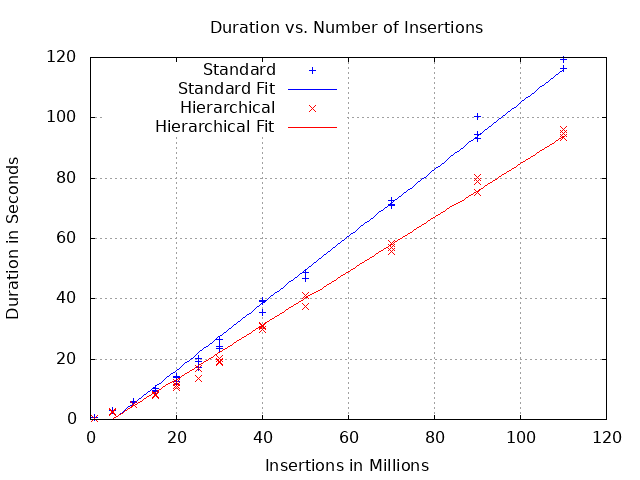
\includegraphics[width=13cm]{scale-nm.png}
\end{center}
The slope of the line of best fits that are plotted are as follows whre $n$ is millions of insertions:
\begin{itemize}
    \item The best fit line for the standard implementation is: $t = (1.1078 \pm 0.01446 )\cdot n - (5.78611   \pm 0.7407)$
    \item The best fit line for the hierarchical implementation is: $t = (0.893221 \pm 0.01166 )\cdot n - (4.52759 \pm 0.597 )$
\end{itemize}
We will disregard the constant as we care about how these data structures perform as input volume scales. We can compute the efficiency difference by dividing the slopes:
$$\text{Hierarchical Implementation Slope}/ \text{Standard Implementation Slope} = \text{Efficiency Difference}$$
$$(0.893221 \pm 0.01166 \text{ seconds/operation}) / (1.1078 \pm 0.01446 \text{ seconds/operation}) = 0.806301679 \approx 80\%$$
In other words, our implementation takes $80\%$ less time per operation to complete. 
Thus, for any time frame, if the standard implementation performs one operation, the hierarchical implementation is expected to perform $1/80\% = 1.25$ operations.
Thus, our experiment shows that the hierarchical implementation performs $25\%$ more operations per second than the standard implementation!

%%%%%%%%%%%%%%%%%%%%%%%%%%%%%%%%%%%%%%%%%%
%%%%%%%%%%%%%%%%%%%%%%%%%%%%%%%%%%%%%%%%%%
%%%%%%%%%%%%%%%%%%%%%%%%%%%%%%%%%%%%%%%%%%

\subsection{Comparing False Positive Rate}

For this experiment, we seek to validate that the hierarchical implementation does not have a worse false positive rate than the standard implementation.
\textbf{Hypothesis: We expect them to have approximately the same false positive rate as the theoeretical expectation discussed earlier.}

\subsubsection{Experimental Settings}

The experiment will run as follows. 
\begin{enumerate}
\item Generate $150,000$ random ``insertion'' keys (of length 16).
\item Generate $150,000$ random ``false'' keys to query distinct from the insertion keys (of length 15).
\item For each implementaiton run the following procedure:
\begin{enumerate}
    \item Let $BPE$ be the bits per element (e.g $BPE = 1$ or $BPE = 10$).
    \item Generate a bloom filter of size $150,000\cdot BPE$.
    \item Insert all the `insertion'' keys and query all the ``false'' keys and measure how many of them the bloom filter return as being a member. Report this number.
    \item Repeat for various values of $BPE$.
\end{enumerate}
\item Repeat this procedure again $3$ times with different insertion and false keys.
\end{enumerate}

\subsubsection{Results}
\begin{center}
    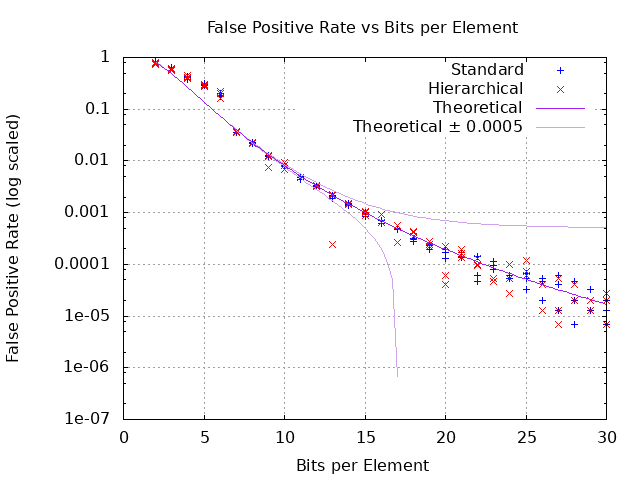
\includegraphics[width=14cm]{fp.png}
\end{center}

As we can see, both the standard and hierarchical implementation closely match the theoeretical expectation. 
Both implementations do worse than theoeretically expected if bloom filters are overpacked, but after Bits per Elements is greater than 6, both implementations are very close to theoeretical expectation ($\pm 0.0005$) or better.

\subsection{Conclusion}
Our experiments have supported both of our theoretically justified hypothesises.
We have demonstrated that the hierarchical implementation is more efficient than the standard implementation; it can perform $25\%$ more operations per second!
Additionally, we have verified our that our implementation is just as effective as the standard implementation. 


	% \section{Application}
	% We will now compare the standard and hierarchical implementation against a real data set.
A common application of networks is in caching queries. Thus, we will use AOL data, which is a collection of query data \cite{AOL} posted by Professor Gregory Dudek.
We will run an experiment to compare the throughput and false positive rate of the standard and hierarchical implementation.
\textbf{Hypothesis: The hierarchical implementaiton will have a higher throughput while maintaing the same false positive rate as the standard implementation.}
\subsection{Experimental Settings}
For this experiment, we will extract out all 736,967 unique queries in the dataset.
We will randomly select 700,000 to insert, and the remaining 36,967 we will use to test the false positive rate.
Generate a bloom filter of both varients with size $BPE\times 730,000$ and insert all $730,000$ selected elements.
Time how long this process takes for each implementaiton . Then query both implementations with the remaining $6,967$ keys to measure the false positive rate.
Do this process for $BPE = 1, 2, 3, \cdots 30$ and plot the results.

\subsection{Results}
\begin{center}
    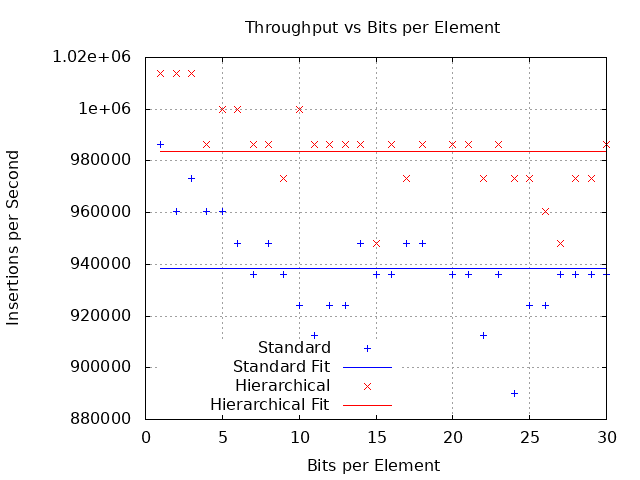
\includegraphics[width=14cm]{aol_thru.png}
\end{center}

As we can see, the hierarchical implementation does noticably better than the standard implementation. 
The lines shown on the graph represents the line of best fit for the function $f(BPE) = c$. In otherwords, it represents an ``average'' throughput for each implementation.
The average throughput for the standard implementation is $938,248$ while the averge throughput for the hierarchical implementaion is $983,627$.
Our hierarchical implementation has a higher throughput by $4\%$! This difference is not as high as it was for the random data since we have many fewer entries.
The hierarchical implementation is more beneficial the more memory is used, since higher memory usage increases the liklihood of page faulting, which is considerably more harmful in the standard implementation.
However, even for smaller uses, our implementation outpaces the standard implementation!

\begin{center}
    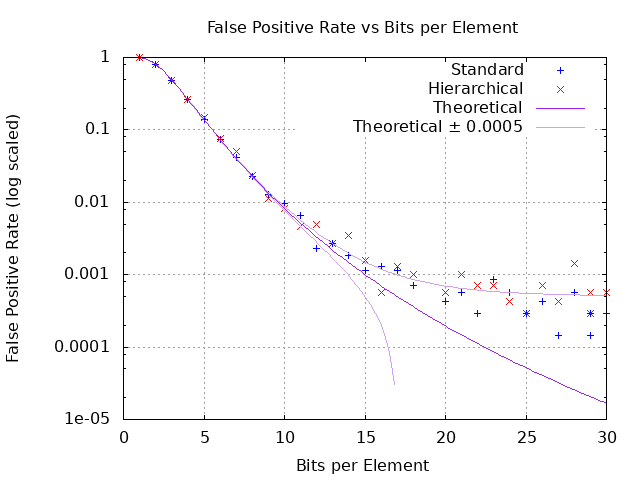
\includegraphics[width=14cm]{aol_fp.png}
\end{center}

Notice that both implementations don't perfectly match the theoretical expectation, but this can be mainly attributed to the small sample size we used to measure the false positive rate.
More importantly,the hierarchical and standard implementation have a similar false positive rate. 

\subsection{Conclusion}
Our results are positive and we hav demonstrated that our implementation is more performant without sacrificing any effectiveness.




	\section{Literature Survey}
	% In my literature survey, I discovered a similar approach except making bloom filters hierarchial.
% Tim Kaler's proposed cache-efficient bloom filters \cite{Kaler} makes sub-bloom filters of size cache-size; thus, their idea is very similar to mine except they do it on a smaller unit of memory.

% Evgeni Krimer and Mattan Erez used a power-of-two choice principle within blocked-bloom filters to decrease the false positive rate.
% Instead of simply selecting one block to write into, they choose multiple.
% \cite{Krimer}.


Felix Putze et al. developed bloom filters with better cache efficiency and requiring less hash bits than the standard bloom filter \cite{Putze}.

 

	\section{Conclusion}
	In this paper, we have theoretically and emperically justified a variant implementation of bloom filters
that lead to much higher performance without increasing the false positive rate.
We anaylzed the expected number of unique pages accessed per query, which should coorelate with expected number of page faults, and found that our implementation is expected to page fault less.
Moreover, we found a closed form expression of the false positive rate of our implementaiton and found that it was equivalent to the standard implementation's false positive rate.
Additionally, we performed two experiments with randomly generated keys to emperically back these claims.
Lastly, we compared the standard and hierarchical implementation on a real data set.
Our findings were positive: our implementation is more efficient than the standard implementation while maintaing the same false positive rate.

	\newpage
	\bibliography{refs}
	
\end{document}